\chapter{Consideraciones de Dise\~no}
	\section{Dise\~no de Alto Nivel}
        Desde el punto de vista de la ingenier\'ia, el dise\~no de software es una etapa crucial del desarrollo de software, en la cual sus implicaciones y 
		deficiencias afectan el proyecto a lo largo de su ciclo de vida\cite{pressman}, por lo que la toma de decisiones sobre el dise\~no es una tarea que debe 
		ser llevada a cabo con especial atenci\'on y cuidado.

		La t\'ecnica de dise\~no que se emple\'o fue la denominada Responsibility Driven Design\cite{responsibility}. Esta t\'ecnica de dise\~no fue concebida en 
		el a\~no 1990 con la intenci\'on de cambiar la visi\'on de los objetos como datos y algoritmos por roles y responsabilidades.
		
		Adem\'as, se intent\'o que el dise\~no cumpliese con los principios fundamentales del dise\~no de software, com\'unmente conocidos 
    	por el acr\'onimo ``\textbf{SOLID}''\cite{objmentor} (\textbf{S}ingle Responsability, \textbf{O}pen-Closed, \textbf{L}iskov Substitution, \textbf{I}
    	nterface Segregation y \textbf{D}ependency Inversion). De aplicar estos principios de manera conjunta, hacen m\'as probable que un programador cree un 
    	sistema de f\'acil mantenimiento y extensible en el tiempo.
    	\begin{description}
    		\item \textbf{Single Responsibility Principle (SRP)}: No debe existir m\'as de una raz\'on para que una clase cambie. Esto significa que una clase con 
    		diferentes responsabilidades debe ser dividida en clases m\'as simples.
    		\item \textbf{Open-Closed Principle (OCP)}: Este principio establece que las entidades de software (clases, m\'odulos, funciones, etc.) deben estar 
    		abiertas para su extensi\'on pero cerradas para su modificaci\'on\cite{oosc}.
    		\item \textbf{Liskov Substitution Principle (LSP)}: Aquellas funciones que usan punteros o referencias a clases base deben ser capaces de utilizar 
    		objetos de clases derivadas, sin saberlo. Barbara Liskov lo describi\'o unos 8 a\~nos antes\footnote{Barbara Liskov, ``Data Abstraction and 
    		Hierarchy'' (Mayo de 1988).} como:
    		\begin{quote}
    		\textit{Lo que se intenta aqu\'i es algo como la siguiente propiedad de sustituci\'on: Si para cada objeto o$_1$ de tipo S existe un objeto o$_2$ de 
    		tipo T tal que para todos los programas P definidos en t\'ermino de T, el comportamiento de P no se ve alterado cuando o$_1$ es sustituido por o$_2$, 
    		entonces S es un subtipo de T.}
    		\end{quote}
    		\item \textbf{Interface Segregation Principle (ISP)}: Los clientes no deben ser forzados a depender de interfaces que no usan, lo que puede ser 
    		interpretado como el hecho de que las interfaces deben tener usuarios que las usen de manera completa, no parcial. Si este \'ultimo fuese el caso, 
    		entonces debe haber otra interfaz con el subconjunto de m\'etodos que este usuario particular necesita.
    		\item \textbf{Dependency Inversion Principle (DIP)}: Este principio establece dos puntos:
    		\begin{itemize}
    			\item M\'odulos de alto nivel no deben depender de m\'odulos de nivel m\'as bajo. Ambos deben depender de abstracciones.
    			\item Abstracciones no deben depender de los detalles. Los detalles deben depender de las abstracciones.
    		\end{itemize}	
    	\end{description}
	
		Observando el nuevo diagrama al estilo OSI del framework \fud (\ref{redisenioFud}) se puede observar claramente que el dise\~no se divide en dos partes, 
		aplicaciones cliente y servidor. A su vez, cada una de estas partes se encuentra organizada en 5 capas separadas, donde cada una de ellas posee una 
		responsabilidad bien definida.
		
		Cabe destacar que el \'unico enlace \textit{real} entre las aplicaciones cliente y servidor estar\'a en el nivel m\'as bajo, es decir, en alguna 
		implementaci\'on del middleware de distribuci\'on. Las restantes formas de comunicaci\'on son abstractas y deben atravesar la estructura de capas.

    \subsection{Application Layer (L5)}\label{applicationLayer5}
			La capa de aplicaci\'on provee los componentes que contienen todos los aspectos del problema a resolver. Entre estos aspectos se incluyen 
			todas las definiciones de los datos que se usan y la manipulaci\'on de los mismos, como as\'i tambi\'en, los algoritmos relevantes para la 
			soluci\'on del problema.

			Es necesario aclarar que, bajo ning\'un punto de vista, esta capa forma parte del framework \fud. Como cualquier c\'odigo de aplicaci\'on que hace
			uso de una biblioteca no forma parte de la misma. Sin embargo, la inclusi\'on de esta capa tiene como principal objetivo servir de ayuda para la 
			comprensi\'on del funcionamiento de la biblioteca.
			
			Las responsabilidades de esta capa son:
			\begin{description}
				\item \textbf{Lado Servidor}: Proveer a la capa subyacente el nodo/estado inicial de la aplicaci\'on junto con la colecci\'on de elementos
				sobre la cual operar\'a el motor combinatorio. Adem\'as, debe definir qu\'e hacer una vez que arribe 
				un paquete resultado.

				\item \textbf{Lado Cliente}: Proveer la \textit{deserializaci\'on} de un nodo. En \ref{mili} mencionamos el gran uso que se le da a 
				MiLi en este proyecto, par\-ti\-cu\-lar\-men\-te a los \textit{binary streams}. Estos se utilizan para la \textit{se\-ria\-li\-za\-ci\'on} 
				y \textit{deserializaci\'on} de los paquetes que viajan desde el servidor hacia los clientes y viceversa. Serializaci\'on es el proceso de 
				convertir una estructura de datos o un objeto en un formato que pueda ser almacenado (como por ejemplo un archivo, o un buffer de memoria) o 
				transmitido a trav\'es de una conexi\'on de red para m\'as tarde, probablemente en otra computadora, realizar el proceso inverso, ``resucitar'' el 
        objeto o estructura original\footnote{\url{http://en.wikipedia.org/wiki/Serialization}}.
				\item \textbf{Com\'un a Ambos Lados}: Se deben proveer, a la capa L4, las pol\'iticas de Combinaci\'on y de Poda (son las que determinan el 
				comportamiento del motor combinatorio).
				
				Adem\'as, se necesita definir el nodo de la aplicaci\'on, detallando, entre otras cosas, qu\'e informaci\'on contendr\'a y c\'omo se llevar\'a a cabo su serializaci\'on. 
				Como se mencion\'o en \ref{nodoL4}, el nodo representa un estado durante la ejecuci\'on y es lo que el servidor distribuye entre los clientes para 
				su procesamiento.
			\end{description}
%% 			Una vez terminado todo lo anterior, se proceder\'a al m\'etodo \textit{main}, el cual entre sus l\'ineas deber\'a tener algunas fundamentales:
%% 			\begin{table}[!htb]
%% 				\lstset{language=C++}
%% 				\begin{lstlisting}[frame=single]
%% /* ... */
%% 
%% int main(int argc, char** argv)
%% {
%% 	/* ... */
%% 
%% 	auto_ptr <recabs::RecursionManager> _manager(new recabs::PrototypeRM(server, client));
%%     _manager->start();
%%     
%% 	/* ... */    
%% }
%% /* ... */
%%         		\end{lstlisting}
%%         		\centering \caption{Creaci\'on y ejecuci\'on de RecursionManager.} 
%%         		\label{recursionManager}
%%         \end{table}
%% 
%% 			Primero se crea una instancia de \texttt{RecursionManager}, que recibe como par\'ametro las instancias de las aplicaciones cliente y servidor (las 
%% 			implementaciones de las interfaces L5ApplicationClient y L5ApplicationServer, respectivamente). RecursionManager forma parte de \recabs \ y es el 
%% 			encargado de administrar la recursi\'on encarg\'andose de los paquetes que salen y que entran. Luego se lo pone a correr invocando su m\'etodo 
%% 			``\texttt{start()}'' (para m\'as informaci\'on, ir a \ref{recabs}). 

	\newpage	
  \subsection{Combinatory Engine (L4)}
			Esta capa es la que provee la estructura para definir soluciones a problemas que requieren un motor combinatorio.\newline
			Entre sus responsabilidades se encuentran:
			\begin{description}
				\item \textbf{Lado Servidor:} Proveer a la capa subyacente el functor recursivo inicial\footnote{el functor recursivo no es m\'as que el nodo 
				inicial que L5 provee a L4, con la diferencia de que el primero se encuentra serializado} del problema y definir los pasos a seguir cada vez que 
				se recibe un paquete de resultado.
				
				\item \textbf{Lado Cliente:} Proveer la deserializaci\'on de un functor recursivo.
				\item \textbf{Com\'un a Ambos Lados:} Se debe proveer la serializaci\'on de un functor recursivo y la definici\'on de la funci\'on \textit{call}.
				Esta funci\'on es la que debe especificar c\'omo un functor recursivo debe generar sus hijos (estados siguientes), retorn\'andolos en una lista de 
				functores.
				
				Dependiendo en que etapa se encuentre un functor, se ejecuta
				\begin{itemize}
					\item \textit{un caso base:} devolver un resultado, o
					\item \textit{un caso inductivo:} llenar la lista de functores hijos.
				\end{itemize}
				De este modo, la representaci\'on de cualquier funci\'on recursiva solo pasa por la implementaci\'on de la clase abstracta 
        \emph{SerializableRecursiveFunctor} de \recabs, especificando la manera en que se deben generar los hijos.
			\end{description}

			Notar que entre \combeng \ y \recabs \ hay ciertas responsabilidades que, si bien operan sobre diferentes tipos de instancias, se repiten. Tales son 
			los casos de la serializaci\'on/deserializaci\'on de un nodo (o functor) o la de proveer el nodo (o functor) inicial. Lo que sucede es 
			que \combeng, la capa 4, no conoce absolutamente nada del dominio del problema por lo que no sabe como realizar la serializaci\'on de un nodo, o que 
			objetos iniciales proveer al motor combinatorio. Entonces, esta capa act\'ua como un puente derivando aquellas tareas que no conoce a la capa 
			superior. De esta manera, ocurren relaciones de herencia en tres niveles. Todo esto se aclarar\'a a continuaci\'on, en Disen\~no de Bajo Nivel.
			
			\begin{center}
%%             	\begin{figure}
%%     	            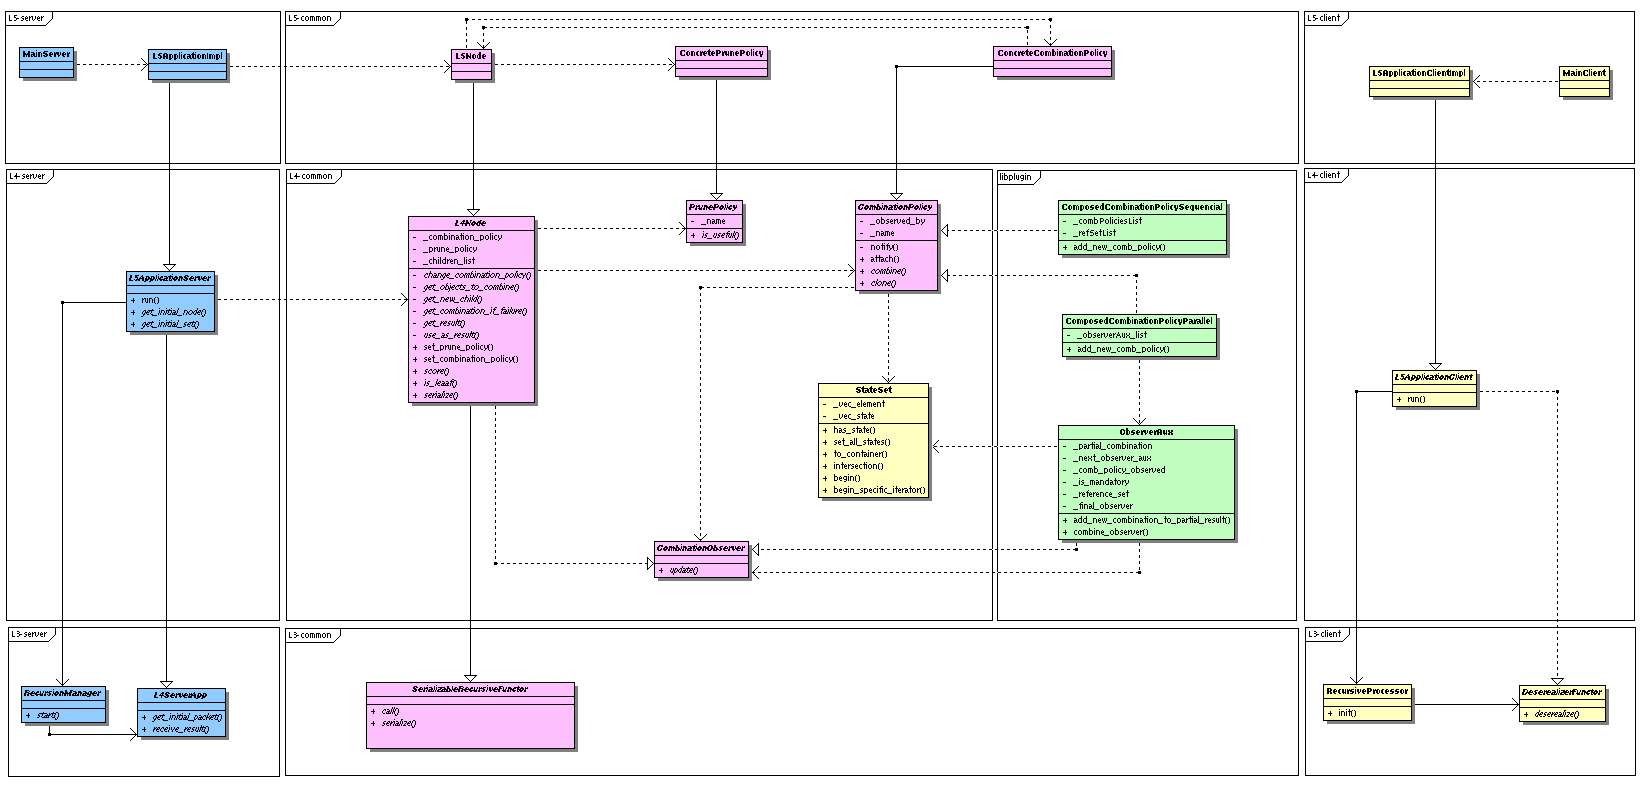
\includegraphics[width=2\textwidth, angle=270]{images/classDiagram.png}
%% 	                \caption{Diagrama de Clases de \combeng \ y sus capas inmediatas}
%% 	                \label{redisenioFud}
%%                 \end{figure}
                \begin{landscape}
               	\begin{figure}
    	            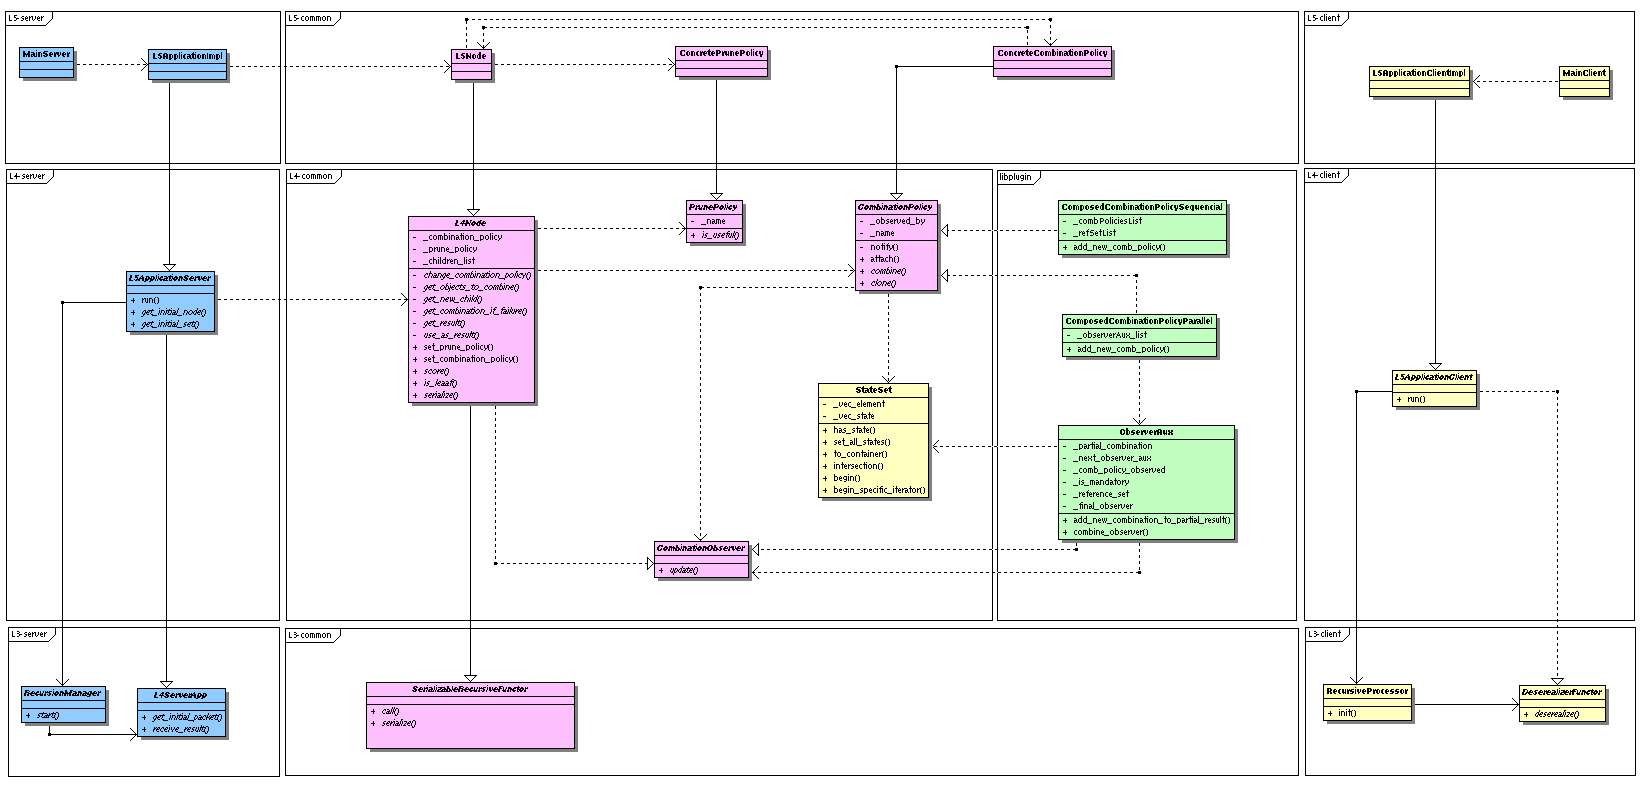
\includegraphics[scale=.36]{images/classDiagram.png}
	                \caption{Diagrama de Clases de \combeng \ y sus capas inmediatas}
	                \label{classDiagram}
                \end{figure}
                \end{landscape}
        	\end{center}
		
	\section{Dise\~no de Bajo Nivel}
		Aqu\'i se hace un refinamiento de las decisiones de dise\~no sobre aquellos componentes abstractos presentes en el dise\~no de 
		alto nivel. Adem\'as, se analiza c\'omo estas clases est\'an compuestas: los atributos de cada una, los m\'etodos que declaran y sus interacciones con el resto del sistema.
		
		Sin entrar en mucho detalle sobre las decisiones de dise\~no que se tuvieron en cuenta sobre cada m\'odulo, se examina, a continuaci\'on, la capa 
		\combeng . Para cada componente del m\'odulo se muestra un diagrama de clases simplificado.
		
		\subsection{\texttt{L4node}}
			En la secci\'on \ref{nodoL4} solo se hab\'ia hecho menci\'on a un nodo de \combeng \ como un concepto abstracto de estado de una aplicaci\'on, pero 
			como se puede observar en la figura \ref{l4NodeClass}, \texttt{L4Node} hereda de \texttt{CombinationObserver} y \texttt{SerializableRecursiveFunctor}, 
			satisfaciendo otros dos roles que se explican a continuaci\'on:
			\begin{itemize}
				\item\textit{L4Node es un observador:} el nodo observa a la pol\'itica de combinaci\'on. 
				Por cada nueva combinaci\'on que la pol\'itica del nodo corriente genere, \'este ser\'a notificado y evaluar\'a, mediante su pol\'itica de poda,
        si dicha combinaci\'on es \'util. En caso afirmativo, crear\'a un nuevo nodo del nivel 5 (de ahora en m\'as lo llamaremos \texttt{L5Node}) y lo
        pondr\'a en su lista de hijos (\texttt{\_children\_list}).
				\item\textit{L4Node es un functor recursivo:} para ello, el nodo del nivel 4 debe implementar los m\'etodos que \texttt
				{SerializableRecursiveFunctor} define en el nivel 3, que son los m\'etodos \texttt{call} y \texttt{serialize}.
				\begin{description}
					\item \footnotesize{\texttt{void serialize(recabs::Packet\& pkt)}}
					
					\normalsize Este m\'etodo, por razones obvias de que el nodo en L4 no posee ning\'un tipo de informaci\'on \'util para la aplicaci\'on, es 
					imposible brindar alg\'un modo de serializaci\'on que resulte de utilidad. Debido a \'esto, quien lo implementa es \texttt{L5Node}.
					
					\item \footnotesize{\texttt{void call(recabs::ChildrenFunctors\& children, recabs::Packet\& result)}}
					
					\normalsize \texttt{call} est\'a implementado usando los m\'etodos virtuales definidos en esta clase, dado que, al igual que la 
					serializaci\'on, en la capa 4 no se tiene informaci\'on suficiente sobre el dominio del problema. En la figura \ref{SDcall} se muestra un 
					diagrama de secuencia exhibiendo el comportamiento de este m\'etodo.
          \begin{figure}[H]\hspace{-.9cm}
    			 	    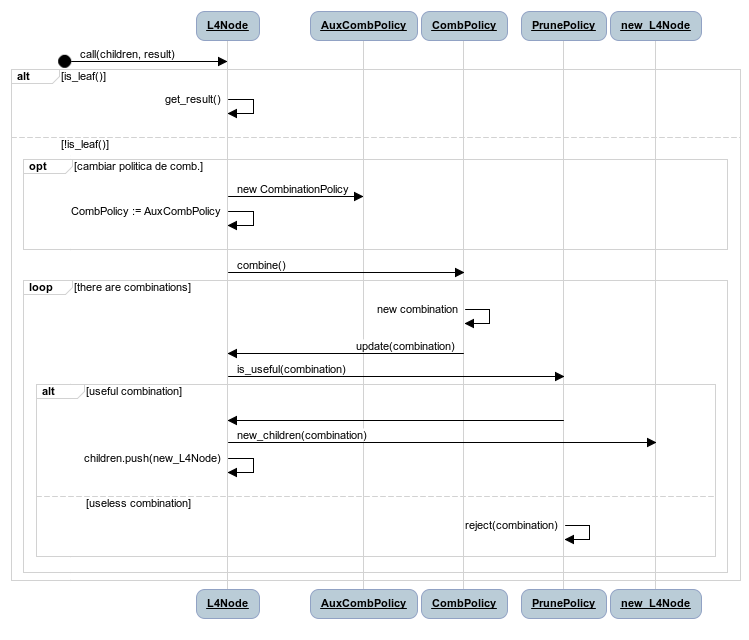
\includegraphics[scale=.6]{images/Call_SeqDiagram.png}
		                \caption{Diagrama de Secuencia del M\'etodo \texttt{call}.}
				    \label{SDcall}
        	\end{figure}
          \vspace{-.6cm}
				\end{description}
				\item \textit{L4Node es un estado de aplicaci\'on:} adem\'as de la serializaci\'on, el desarrollador de la aplicaci\'on debe implementar los 
				siguientes m\'etodos en su L5Node:
				\begin{itemize}
            \scriptsize{}
					\item \texttt{void new\_children(const std::list<T>\&  combination, std::list<L4Node*>\&)}
					\item \texttt{float score()}
					\item \texttt{CombinationPolicy<T>* get\_combination\_if\_failure(const std::string\& failed\_comb\_policy)}
					\item \texttt{CombinationPolicy<T>* change\_combination\_policy()}
					\item \texttt{bool use\_as\_result()}
					\item \texttt{recabs::Packet get\_result()}
					\item \texttt{void get\_objects\_to\_combine(std::list<T>\&)}
					\item \texttt{bool is\_leaf()}
					\item \texttt{void serialize(recabs::Packet\& pkt)}
				\end{itemize}
			\end{itemize}
			\begin{figure}[H] \hspace{.65cm}
    	 	    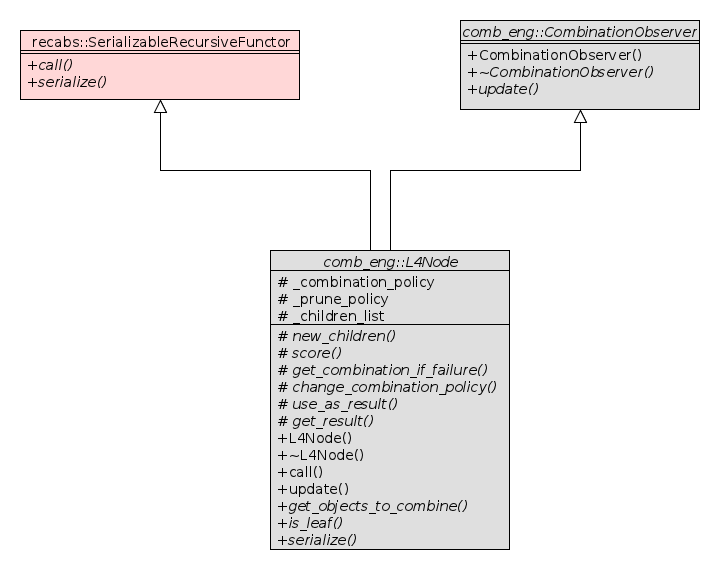
\includegraphics[scale=.46]{images/l4node_class.png}
		        \caption{Clase \texttt{L4Node}.}
		        \label{l4NodeClass}
            \end{figure}

		\subsection{\texttt{PrunePolicy}}
			La pol\'itica de poda es la que define si una combinaci\'on es de utilidad o no. El desarrollador de la aplicaci\'on deber\'a implementar en su 
			pol\'itica de poda concreta el \'unico m\'etodo definido por la interfaz que se observa en la figura \ref{prunePolicyClass}:
			\begin{itemize}
				\item[-] \footnotesize{\texttt{bool is\_useful(const std::list<T>  combination)}}
			\end{itemize}			
			\begin{figure}[H]\hspace{4cm}
   	   	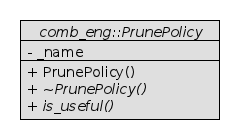
\includegraphics[scale=.56]{images/prune_policy_class.png}
	      \caption{\texttt{PrunePolicy} class}
	      \label{prunePolicyClass}
       \end{figure}

		\subsection{\texttt{CombinationObserver}}
      Para las pol\'iticas de combinaci\'on se utiliz\'o el patr\'on de dise\~no \textit{Observer} (\textit{ve\'ase} \ref{patron_observer}). Como se
      mencion\'o anteriormente, \texttt{L4Node} es un observador de una pol\'itica, por lo que el mismo deber\'a implementar el m\'etodo update
      definido en CombinationObserver:
      \begin{description}
        \item \texttt{void update(const std::list<T>\& combination)}
      \end{description}
				\begin{figure}[H] \hspace{3.6cm}
    	   	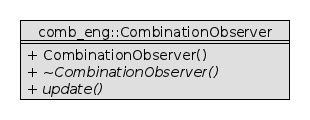
\includegraphics[scale=.56]{images/combination_observer_class.png}
          \caption{Clase \texttt{CombinationObserver}.}
		      \label{combObserverClass}
        \end{figure}
		\subsection{\texttt{CombinationPolicy}}
			La pol\'itica de combinaci\'on es la que define la forma en que una colecci\'on de elementos ser\'an combinados. El desarrollador deber\'a implementar 
			en su pol\'itica de combinaci\'on concreta, los m\'etodos de la interfaz que se observan en la figura \ref{combPolicyClass}:
			\begin{itemize}
				\item[-] \footnotesize{\texttt{void combine(const std::list<T>\&  objects\_to\_combine, Status\& combination\_status)}}. \normalsize{}Como su nombre 
				  lo indica, es el que determina el comportamiento de la pol\'itica, c\'omo se generan las combinaciones. Posee dos argumentos, el primero es la 
				  colecci\'on de elementos que debe combinar y el segundo es el estado con el que finaliza.
				\item[-] \footnotesize{\texttt{CombinationPolicy<T>* clone (CombinationObserver<T>* obs)}}.\\ 
				  \normalsize Retorna una nueva instancia id\'entica a la pol\'itica de combinaci\'on sobre la cual se invoca.
	
			\end{itemize}
			\begin{figure}[ht] \hspace{3.6cm}
    	  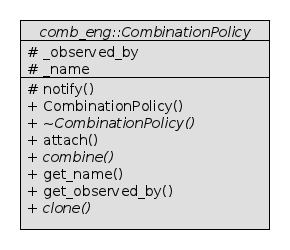
\includegraphics[scale=.56]{images/combination_policy_class.png}
		    \caption{\texttt{CombinationPolicy} class}
		    \label{combPolicyClass}
      \end{figure}
      \subsubsection{Pol\'iticas De Combinaci\'on Provistas Por \combeng}
      	Durante el desarrollo de las aplicaciones que se incluyen en este proyecto se han implementado 
      	diferentes pol\'iticas de combinaci\'on, algunas \textit{simples} y otras \textit{compuestas}. Las simples son algoritmos combinadores propiamente 
      	dichos, mientras que las compuestas combinan a dos o m\'as pol\'iticas simples. Estas \'ultimas no generan combinaciones por s\'i mismas, son las 
      	simples quienes se encargan de obtenerlas.
        		
      	Dentro de las simples, est\'an:
      	\begin{itemize}
          \item \texttt{ListCombinationPolicy}\label{listCombPolicy}: Esta pol\'itica retornar\'a uno a uno los elementos a combinar. El argumento
            \texttt{combination\_status} informar\'a un fallo si el conjunto de elementos se encuentra vac\'io.
      		\item \texttt{NewtonianCombinationPolicy}: el m\'etodo \texttt{combine} de esta pol\'itica implementa el cl\'asico algoritmo que retorna
       			todos los subconjuntos de tama\~no K, con \emph{MIN$\leq$K$\geq$MAX} \footnote{MIN y MAX son establecidos por el usuario}. El \texttt{combination\_status} 
			informa la ocurrencia de un fallo en caso de que la cantidad de elementos a combinar sea sea cero o menor a \emph{MIN}.
       			
      	\end{itemize}
        Mientras que de las compuestas hay otras dos:\label{composedCombinationPolicies}
      	\begin{itemize}
	    		\item \texttt{ComposedCombinationPolicySequencial}: Esta pol\'itica establece una especie de nexo entre diferentes algoritmos combinatorios. 
	     			B\'asicamente, toma un conjunto de combinadores y los hace combinar en secuencia, uno despu\'es de otro. Podr\'ia pensarse como una cola 
	     			(FIFO) de combinadores, el primero en ingresar a la cola es el primero en combinar.
	     				\begin{figure}[H]\hspace{.8cm}
	     					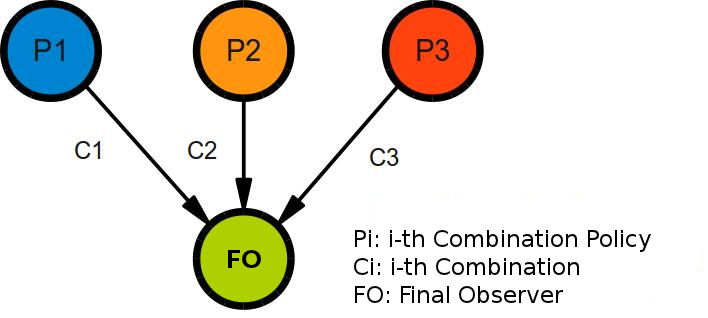
\includegraphics[scale=.45]{images/Comb1.jpg}
	     					\caption{Pol\'itica de Combinaci\'on Compuesta Secuencial.}
	     				\end{figure}
            \item \texttt{ComposedCombinationPolicyParallel}\label{composedCombPolicyParallel}: Esta pol\'itica toma un grupo de algoritmos combinadores
              (pol\'iticas simples) y los pone a ``correr'' en paralelo. Es decir, cada combinaci\'on que genera la primer pol\'itica se une con cada
              combinaci\'on generada por la segunda y as\'i sucesivamente, hasta llegar a la \'ultima de \'estas, la cual har\'a entrega de todo el 
              paquete al observador final.
      			\begin{figure}[H]\hspace{.3cm}
	     				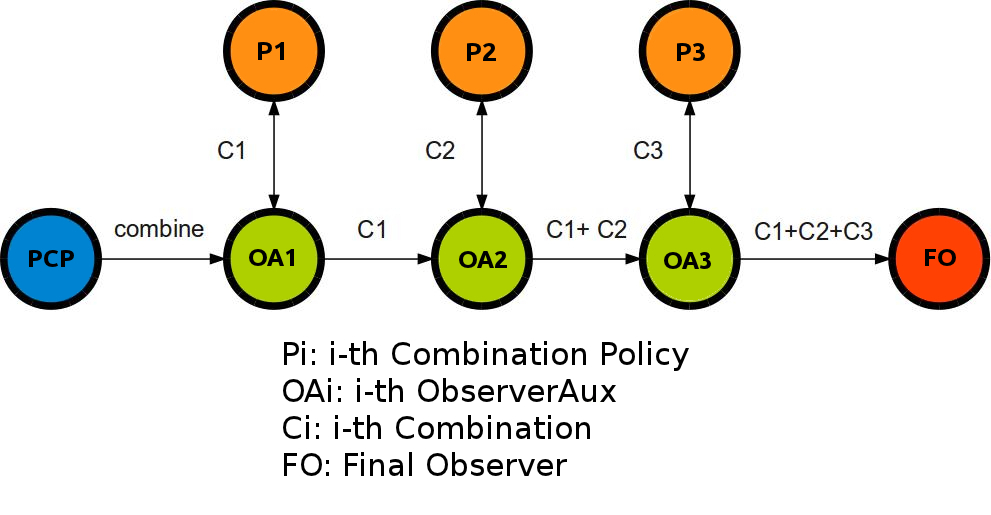
\includegraphics[scale=.4]{images/Comb2.jpg}
	     				\caption{Pol\'itica de Combinaci\'on Compuesta Paralela.}
              \label{parallelComb}
	     			\end{figure}
            \newpage
            De la Figura \ref{parallelComb} se puede observar la nueva entidad \textit{ObserverAux} la cual realiza, repetitivamente hasta que no
            reciba m\'as combinaciones, las siguientes tareas:
            \begin{itemize}
              \item Recibir una combinaci\'on generada por la pol\'itica que observa.
              \item Unir dicha combinaci\'on con aquella que proviene del observador auxiliar anterior, siempre y cuando no se trate del primer
                algoritmo combinatorio (\textbf{P1}). 
              \item Entregar la uni\'on al observador auxiliar de la siguiente primitiva simple. 
            \end{itemize}
            \begin{figure}[H]\hspace{2.8cm}
              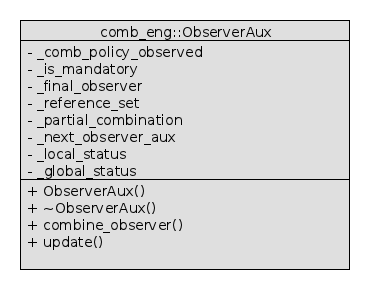
\includegraphics[scale=.6]{images/observer_aux_class.png}
              \caption{Clase \texttt{ObserverAux}.}
              \label{observerAux}
            \end{figure}
            A partir de la figura anterior, se explican cada uno de sus atributos:
            \begin{description}
              \item \texttt{\_comb\_policy\_observed}: tal y como su nombre lo indica, es la pol\'itica a la que se esta observando.
              \item \texttt{\_is\_mandatory}: a la hora de la creaci\'on de una nueva instancia de un ObserverAux, es necesario establecer si la misma ser\'a
                mandatoria o no. Cada una de las pol\'iticas simples opera sobre un conjunto de elementos (\_reference\_set) no necesariamente igual al resto,
                por lo que si una de las pol\'iticas falla (por ejemplo, no dispone de mas combinaciones) y es mandatoria, toda la pol\'itica compuesta
                fallar\'a. Por otro lado, si la misma no es mandatoria implica que este observador auxiliar act\'ue como un ``puente'', dejando
                pasar aquellas uniones que provienen de las primitivas anteriores a siguiente observador.
              \item \texttt{\_partial\_combination}: es la combinaci\'on que recibe del observador auxiliar anterior a \'el. En el caso de que sea el primero,
                este atributo estar\'a vac\'io.
              \item \texttt{\_next\_observer\_aux}: es aquel al que se le debe entregar la combinaci\'on parcial.
              \item \texttt{\_global\_status} y \texttt{\_local\_status} son los que permiten llevar el estado de la pol\'itica compuesta y de cada una de las
                primitivas simples, respectivamente.
            \end{description}
      		\end{itemize}
        	
		\subsection{\texttt{L5ApplicationServer}}
		L5ApplicationServer constituye el lado servidor de la aplicaci\'on. Quien desarrolle una aplicaci\'on sobre \combeng, deber\'a implementar, al menos, los siguientes m\'etodos:
		\begin {description}
		  \item \texttt {get\_initial\_packet}: Retorna un paquete de datos representando al nodo inicial de la aplicaci\'on. Dicho nodo es enviado a un cliente, para que sea \'el quien inicie la ejecuci\'on de la aplicaci\'on.
		  \item \texttt {receive\_result}: Durante el procesamiento de un nodo, los clientes pueden enviar resultados al servidor. Este m\'etodo es quien decide qu\'e hacer con los mismos.
		\end {description}


			\begin{figure}[H] \hspace{3.6cm}
       	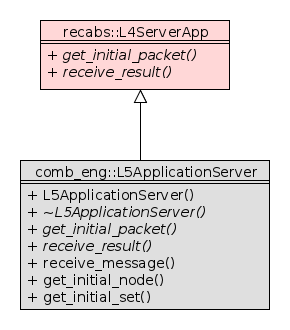
\includegraphics[scale=.56]{images/l5app_server_class.png}
        \caption{Clase \texttt{L5ApplicationServer}.}
        \label{l5AppServerClass}
 	    \end{figure}
        	
		\subsection{\texttt{L5ApplicationClient}}
		L5ApplicationClient constituye el lado cliente de la aplicaci\'on. El desarrollador deber\'a proveer la implementaci\'on de la \'unica funcionalidad requerida por \combeng:
  		\begin {description}
		  \item \texttt {deserialize}: Este m\'etodo efect\'ua el proceso de conversi\'on de un paquete que viaja por la red (\emph {binary-stream}) a un nodo utilizable por la aplicaci\'on. 
		\end {description}


			\begin{figure}[H] \hspace{3.6cm}
        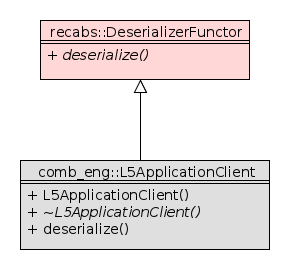
\includegraphics[scale=.56]{images/l5app_client_class.png}
        \caption{Clase \texttt{L5ApplicationClient}.}
        \label{l5AppClientClass}
 	    \end{figure}
